\documentclass[]{article}
\usepackage{lmodern}
\usepackage{amssymb,amsmath}
\usepackage{ifxetex,ifluatex}
\usepackage{fixltx2e} % provides \textsubscript
\ifnum 0\ifxetex 1\fi\ifluatex 1\fi=0 % if pdftex
  \usepackage[T1]{fontenc}
  \usepackage[utf8]{inputenc}
\else % if luatex or xelatex
  \ifxetex
    \usepackage{mathspec}
    \usepackage{xltxtra,xunicode}
  \else
    \usepackage{fontspec}
  \fi
  \defaultfontfeatures{Mapping=tex-text,Scale=MatchLowercase}
  \newcommand{\euro}{€}
\fi
% use upquote if available, for straight quotes in verbatim environments
\IfFileExists{upquote.sty}{\usepackage{upquote}}{}
% use microtype if available
\IfFileExists{microtype.sty}{%
\usepackage{microtype}
\UseMicrotypeSet[protrusion]{basicmath} % disable protrusion for tt fonts
}{}
\usepackage[margin=1in]{geometry}
\usepackage{color}
\usepackage{fancyvrb}
\newcommand{\VerbBar}{|}
\newcommand{\VERB}{\Verb[commandchars=\\\{\}]}
\DefineVerbatimEnvironment{Highlighting}{Verbatim}{commandchars=\\\{\}}
% Add ',fontsize=\small' for more characters per line
\usepackage{framed}
\definecolor{shadecolor}{RGB}{248,248,248}
\newenvironment{Shaded}{\begin{snugshade}}{\end{snugshade}}
\newcommand{\KeywordTok}[1]{\textcolor[rgb]{0.13,0.29,0.53}{\textbf{{#1}}}}
\newcommand{\DataTypeTok}[1]{\textcolor[rgb]{0.13,0.29,0.53}{{#1}}}
\newcommand{\DecValTok}[1]{\textcolor[rgb]{0.00,0.00,0.81}{{#1}}}
\newcommand{\BaseNTok}[1]{\textcolor[rgb]{0.00,0.00,0.81}{{#1}}}
\newcommand{\FloatTok}[1]{\textcolor[rgb]{0.00,0.00,0.81}{{#1}}}
\newcommand{\CharTok}[1]{\textcolor[rgb]{0.31,0.60,0.02}{{#1}}}
\newcommand{\StringTok}[1]{\textcolor[rgb]{0.31,0.60,0.02}{{#1}}}
\newcommand{\CommentTok}[1]{\textcolor[rgb]{0.56,0.35,0.01}{\textit{{#1}}}}
\newcommand{\OtherTok}[1]{\textcolor[rgb]{0.56,0.35,0.01}{{#1}}}
\newcommand{\AlertTok}[1]{\textcolor[rgb]{0.94,0.16,0.16}{{#1}}}
\newcommand{\FunctionTok}[1]{\textcolor[rgb]{0.00,0.00,0.00}{{#1}}}
\newcommand{\RegionMarkerTok}[1]{{#1}}
\newcommand{\ErrorTok}[1]{\textbf{{#1}}}
\newcommand{\NormalTok}[1]{{#1}}
\usepackage{graphicx}
\makeatletter
\def\maxwidth{\ifdim\Gin@nat@width>\linewidth\linewidth\else\Gin@nat@width\fi}
\def\maxheight{\ifdim\Gin@nat@height>\textheight\textheight\else\Gin@nat@height\fi}
\makeatother
% Scale images if necessary, so that they will not overflow the page
% margins by default, and it is still possible to overwrite the defaults
% using explicit options in \includegraphics[width, height, ...]{}
\setkeys{Gin}{width=\maxwidth,height=\maxheight,keepaspectratio}
\ifxetex
  \usepackage[setpagesize=false, % page size defined by xetex
              unicode=false, % unicode breaks when used with xetex
              xetex]{hyperref}
\else
  \usepackage[unicode=true]{hyperref}
\fi
\hypersetup{breaklinks=true,
            bookmarks=true,
            pdfauthor={Sebri, JcB},
            pdftitle={Questionnaire étudiant},
            colorlinks=true,
            citecolor=blue,
            urlcolor=blue,
            linkcolor=magenta,
            pdfborder={0 0 0}}
\urlstyle{same}  % don't use monospace font for urls
\setlength{\parindent}{0pt}
\setlength{\parskip}{6pt plus 2pt minus 1pt}
\setlength{\emergencystretch}{3em}  % prevent overfull lines
\setcounter{secnumdepth}{5}

%%% Use protect on footnotes to avoid problems with footnotes in titles
\let\rmarkdownfootnote\footnote%
\def\footnote{\protect\rmarkdownfootnote}

%%% Change title format to be more compact
\usepackage{titling}

% Create subtitle command for use in maketitle
\newcommand{\subtitle}[1]{
  \posttitle{
    \begin{center}\large#1\end{center}
    }
}

\setlength{\droptitle}{-2em}
  \title{Questionnaire étudiant}
  \pretitle{\vspace{\droptitle}\centering\huge}
  \posttitle{\par}
  \author{Sebri, JcB}
  \preauthor{\centering\large\emph}
  \postauthor{\par}
  \predate{\centering\large\emph}
  \postdate{\par}
  \date{19/02/2015}



\begin{document}

\maketitle


{
\hypersetup{linkcolor=black}
\setcounter{tocdepth}{2}
\tableofcontents
}
\section{Questionnaire étudiant}\label{questionnaire-etudiant}

Version du Mon May 4 16:17:41 2015

\begin{verbatim}
 [1] "Etab"    "Etud"    "Q1"      "Q2.1"    "Q2.2"    "Q2.3"    "Q2.4"   
 [8] "Q2.5"    "Q2.6"    "Q2.7"    "Q3.1tpc" "Q3.2sp"  "Q3.3tab" "Q3.4ord"
[15] "Q4.1"    "Q4.2"    "Q4.3"    "Q4.4"    "Q4.5"    "Q4.6"    "Q4.7"   
[22] "Q4.8"    "Q4.9"    "Q4.10"   "Q4.11"   "Q4.12"   "Q4.13"   "Q4.14"  
[29] "Q4.15"   "Q4.16"   "Q5"      "Q6"      "Q7.1"    "Q7.2"    "Q7.3"   
[36] "Q7.4"    "Q7.5"    "Q7.6"    "Q7.7"    "Q7.8"    "Q7.9"    "Q7.10"  
[43] "Q7.11"   "Q7.12"   "Q7.13"   "Q7.14"   "Q7.15"   "Q7.16"   "Q8"     
[50] "Q9"      "Q10"     "Q11"    
\end{verbatim}

Le fichier comporte:

\begin{itemize}
\itemsep1pt\parskip0pt\parsep0pt
\item
  1446 lignes
\item
  52 variables
\end{itemize}

\subsection{Etablissements
participant:}\label{etablissements-participant}

\begin{verbatim}
  B1   B2   C1   C2   C3   E1   H1   H2 HUS1 HUS2 HUS3   M1   M2  Sa1  SV1 
  43   54  120  127  110   58   56   51  162   60  131  146  123   42   79 
 SV2 
  84 
\end{verbatim}

\begin{figure}[htbp]
\centering
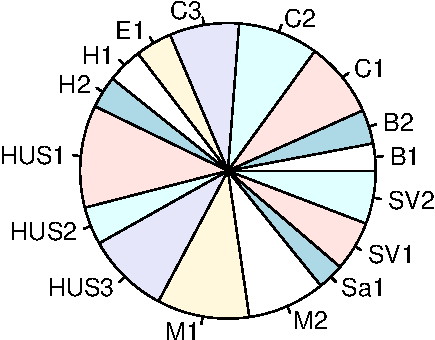
\includegraphics{qs_etudiants_files/figure-latex/participants-1.pdf}
\end{figure}

\subsection{Age}\label{age}

\begin{verbatim}
   Min. 1st Qu.  Median    Mean 3rd Qu.    Max.    NA's 
   17.0    20.0    22.0    24.1    25.0    53.0      27 
\end{verbatim}

\begin{figure}[htbp]
\centering
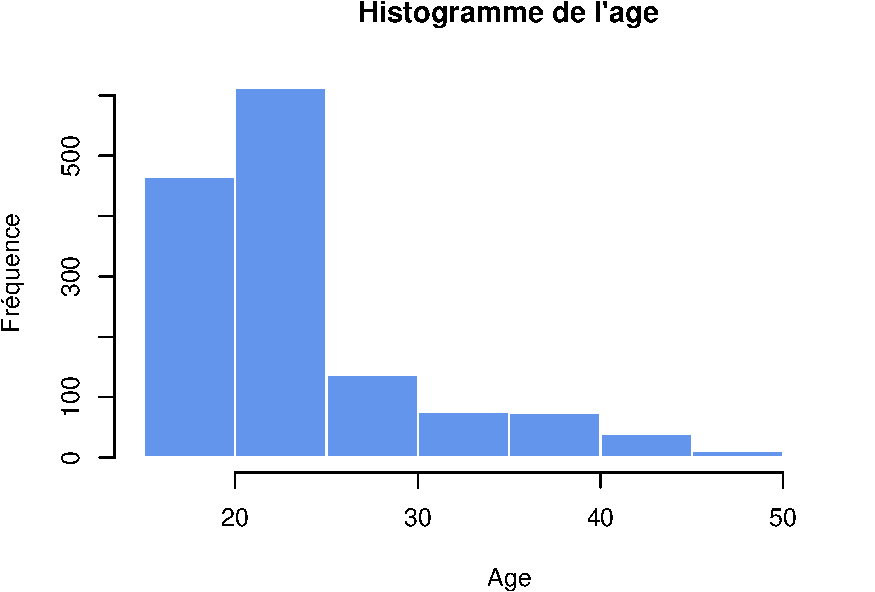
\includegraphics{qs_etudiants_files/figure-latex/age-1.pdf}
\end{figure}

\subsubsection{Générations}\label{generations}

\begin{Shaded}
\begin{Highlighting}[]
\CommentTok{# génération}
\CommentTok{# X = 15 à 20 ans}
\CommentTok{# Y = 20 à 35 ans}
\CommentTok{# Z > 35 ans}

\NormalTok{age <-}\StringTok{ }\KeywordTok{c}\NormalTok{(}\DecValTok{15}\NormalTok{, }\DecValTok{20}\NormalTok{, }\DecValTok{35}\NormalTok{, }\DecValTok{60}\NormalTok{)}
\NormalTok{g <-}\StringTok{ }\KeywordTok{cut}\NormalTok{(d1$Q11, age)}
\KeywordTok{summary}\NormalTok{(g)}
\end{Highlighting}
\end{Shaded}

\begin{verbatim}
## (15,20] (20,35] (35,60]    NA's 
##     466     826     127      27
\end{verbatim}

\begin{Shaded}
\begin{Highlighting}[]
\NormalTok{g2 <-}\StringTok{ }\KeywordTok{cut}\NormalTok{(d1$Q11, age, }\DataTypeTok{labels =} \KeywordTok{c}\NormalTok{(}\StringTok{"X"}\NormalTok{, }\StringTok{"Y"}\NormalTok{, }\StringTok{"Z"}\NormalTok{))}
\KeywordTok{summary}\NormalTok{(g2)}
\end{Highlighting}
\end{Shaded}

\begin{verbatim}
##    X    Y    Z NA's 
##  466  826  127   27
\end{verbatim}

\begin{Shaded}
\begin{Highlighting}[]
\CommentTok{# ajout d'une colonne GENERATION}
\NormalTok{d1$GENERATION <-}\StringTok{ }\NormalTok{g2}
\KeywordTok{factor2table}\NormalTok{(d1$GENERATION)}
\end{Highlighting}
\end{Shaded}

\begin{verbatim}
##                 X      Y      Z  NA's
## nombre     466.00 826.00 127.00 27.00
## proportion  32.23  57.12   8.78  1.87
\end{verbatim}

\begin{Shaded}
\begin{Highlighting}[]
\KeywordTok{barplot}\NormalTok{(}\KeywordTok{summary}\NormalTok{(d1$GENERATION), }\DataTypeTok{xlab =} \StringTok{"Génération"}\NormalTok{, }\DataTypeTok{ylab =} \StringTok{"nombre"}\NormalTok{, }\DataTypeTok{main =} \StringTok{"Répartition des générations au sein des étudiants"}\NormalTok{)}
\end{Highlighting}
\end{Shaded}

\begin{figure}[htbp]
\centering
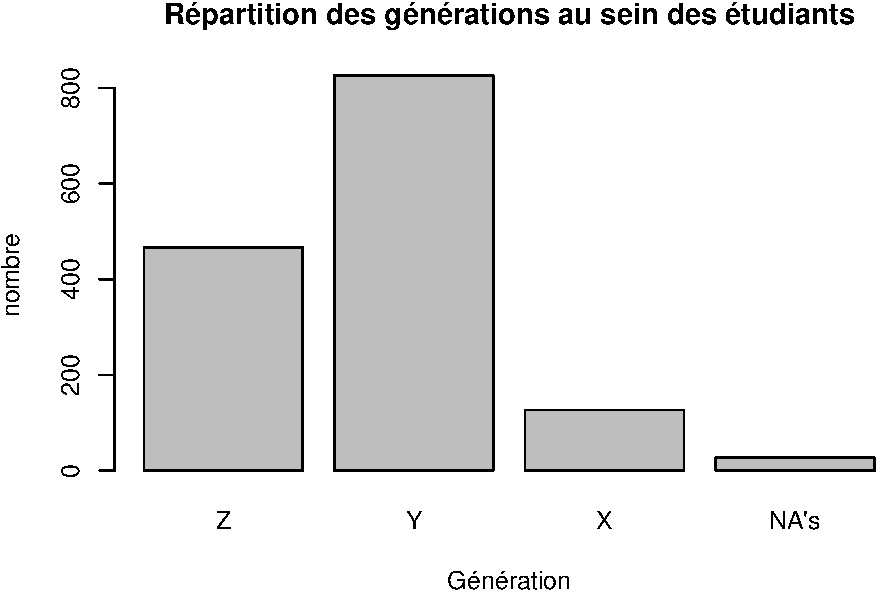
\includegraphics{qs_etudiants_files/figure-latex/generation-1.pdf}
\end{figure}

\subsection{Sexe}\label{sexe}

\begin{verbatim}
   F    H   na NA's 
1218  210    1   17 
\end{verbatim}

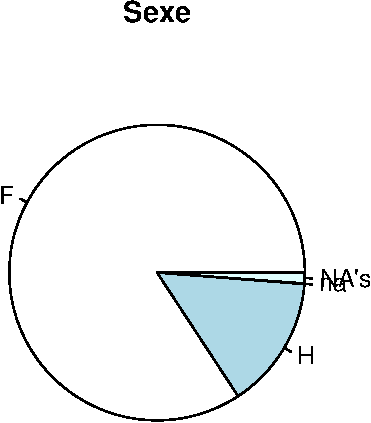
\includegraphics{qs_etudiants_files/figure-latex/sexe-1.pdf} Test de la
routine \textbf{factor2table}

\begin{Shaded}
\begin{Highlighting}[]
\NormalTok{f <-}\StringTok{ }\KeywordTok{factor2table}\NormalTok{(d1$Q10, }\DataTypeTok{digit=}\DecValTok{2}\NormalTok{, }\DataTypeTok{col=}\KeywordTok{c}\NormalTok{(}\StringTok{"femmes"}\NormalTok{,}\StringTok{"hommes"}\NormalTok{,}\StringTok{"inconnu"}\NormalTok{))}
\NormalTok{f}
\end{Highlighting}
\end{Shaded}

\begin{verbatim}
##             femmes hommes inconnu
## nombre     1218.00 210.00   18.00
## proportion   84.23  14.52    1.24
\end{verbatim}

Sous forme de tableau avec \textbf{kable}:

\begin{table}

\caption{Sexe des participants}
\begin{tabular}{l|r|r|r}
\hline
  & femmes & hommes & inconnu\\
\hline
nombre & 1218.00 & 210.00 & 18.00\\
\hline
proportion & 84.23 & 14.52 & 1.24\\
\hline
\end{tabular}
\end{table}

Sous forme de tableau avec \textbf{xtable}:

\% latex table generated in R 3.1.3 by xtable 1.7-4 package \% Mon May 4
16:17:46 2015

\begin{table}[ht]
\centering
\begin{tabular}{rrrr}
  \hline
 & femmes & hommes & inconnu \\ 
  \hline
nombre & 1218.00 & 210.00 & 18.00 \\ 
  proportion & 84.23 & 14.52 & 1.24 \\ 
   \hline
\end{tabular}
\caption{Sexe des participants} 
\label{sexe}
\end{table}

Pie chart
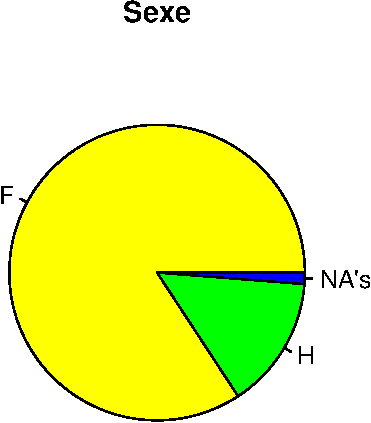
\includegraphics{qs_etudiants_files/figure-latex/pie_sexe-1.pdf}

\subsection{Age et sexe}\label{age-et-sexe}

L'age des hommes et des femmes sont-ils identiques ? On part de
l'hypothèse qu'il n'y a à priori de différence d'age entre les hommes et
les femmes (on appelle cela l'hypothèse nulle ou H0). Si cette hypothèse
est vraie, la différence des moyennes des ages entre les hommes et les
femmes devrait être nulle. En pratique cette différence est rarement
exactement égale à 0 et le problème est de savoir si le chiffre obtenu
est assimilable à 0 ou si on contraire il est trop important pourqu'on
puisse se livrer à cette assimilation, auquel cas on est obligé de
renoncer à l'hypothèse nulle et accepter l'hypothèse alternative: l'age
des hommes est en moyenne différent de celui des femmes. Pour répondre à
la question, on pratique un test statistique pour lequel on défini un
écart par rappport à 0. Si le résultat du test tombe dans l'intervalle
on admet que la différence de moyenne est assimilable à 0 et on accepte
l'hypothèse nulle: pas de différence entre les groupes. Sinon on la
recherche. Bien sûr, plus on défini un intervalle important, plus on
augmente le risque de se tromper en affirmant qu'il n'y a pas de
différence entre les moyennes. C'est ce qu'on appelle le risque de
première espèce ou alpha. Dans les science de la santé, ce risque est
fixé conssenssuellement (et arbitrairement) à 5\% = 5/100 = 0.05 et
généralement rapporté sous la forme p = 0.05 C'est à dire que j'admet H0
(pas de différence) en prenant le risque conssenti de me tromper dans
5\% des cas. En pratique les logiciels calculent la probabilité exacte
d'observer par hasard une telle différence entre les deux groupes. Si
cette probabilité est supérieure à 0.05 (cad comprise entre 0.05 et 1)
on considère que la différence entre les moyennes est un artefact lié au
fluctuation d'échantillonnage et qu'en réalité il n'y a pas de
différence entre les groupes. Si au contraire, la probabilité exacte est
inférieure à 0.05, on admet qu'elle n'est pas due au hasard et on est
obligé d'admettre qu'il y a bien une différence entre les deux groupes.
On voit par là le côté arbitraire du petit p, mais il est considéré dans
toutes les publications comme un chiffre magique\ldots{}

Il existe de nombreux tests statistiques. Pour répondre à la question
posée, on utilise le test t de Student qui s'applique si:

\begin{itemize}
\itemsep1pt\parskip0pt\parsep0pt
\item
  on ne compare que 2 groupes (c'est le cas)
\item
  la variable d'intérêt (ici l'age) suit une loi normale (on va admettre
  que oui) dans les 2 groupes
\item
  la variance (moyenne des écarts à la moyenne) des 2 groupes est égale
  (si ce n'est pas le cas, on peut utiliser une variante de test de
  Student appelée test de Welch).
\end{itemize}

La colonne sexe (Q10) comporte 3 valeurs: H, F et NR. Il faut éliminer
les NR en les transformant en NA pour rendre le test possible

\begin{Shaded}
\begin{Highlighting}[]
\NormalTok{d1$Q10 <-}\StringTok{ }\KeywordTok{toupper}\NormalTok{(d1$Q10)}
\NormalTok{d1$Q10[d1$Q10 ==}\StringTok{ "NR"}\NormalTok{] <-}\StringTok{ }\OtherTok{NA}
\end{Highlighting}
\end{Shaded}

Puis faire le test:

\begin{Shaded}
\begin{Highlighting}[]
\NormalTok{t <-}\StringTok{ }\KeywordTok{t.test}\NormalTok{(d1$Q11 ~}\StringTok{ }\NormalTok{d1$Q10, }\DataTypeTok{var.equal =} \OtherTok{TRUE}\NormalTok{)}
\NormalTok{t}
\end{Highlighting}
\end{Shaded}

\begin{verbatim}
## 
##  Two Sample t-test
## 
## data:  d1$Q11 by d1$Q10
## t = -3.7563, df = 1415, p-value = 0.0001795
## alternative hypothesis: true difference in means is not equal to 0
## 95 percent confidence interval:
##  -2.7497617 -0.8630462
## sample estimates:
## mean in group F mean in group H 
##        23.82645        25.63285
\end{verbatim}

\begin{Shaded}
\begin{Highlighting}[]
\NormalTok{p.t <-}\StringTok{ }\NormalTok{t$p.value}
\end{Highlighting}
\end{Shaded}

On voit que la probabilité exacte d'observer par hasard une telle
différence entre les moyennes est égale à 0.0001795. Cette probabilité
est très inférieure à 0.05 et donc on rejette l'hypothèse d'égalité des
ages. En moyenne, pour cet échantillon, les étudiants hommes sont plus
agés que les étudiantes et cette différence est statistiquement
significative.

Comme on peut avoir un doute sérieux sur la normalité de l'age (voir le
graphique des ages ci-dessus), on réalise un test non paramétrique,
c'est à dire qui ne fait pas d'hypothèse sur la façon dont la variable
est distribuée. Dans le cas particulier on utilise le test de Wilcoxon
qui est l'équivalent non paramétrique du test de Student:

\begin{Shaded}
\begin{Highlighting}[]
\KeywordTok{wilcox.test}\NormalTok{(d1$Q11 ~}\StringTok{ }\NormalTok{d1$Q10)}
\end{Highlighting}
\end{Shaded}

\begin{verbatim}
## 
##  Wilcoxon rank sum test with continuity correction
## 
## data:  d1$Q11 by d1$Q10
## W = 97211, p-value = 0.0000002159
## alternative hypothesis: true location shift is not equal to 0
\end{verbatim}

On arrive à la même conclusion.

\subsection{Q1- Pour ce cours, vous avez pris des
notes}\label{q1--pour-ce-cours-vous-avez-pris-des-notes}

\begin{verbatim}
             ordi papier    pas     X
nombre     410.00 720.00 232.00 84.00
proportion  28.35  49.79  16.04  5.81
\end{verbatim}

\begin{figure}[htbp]
\centering
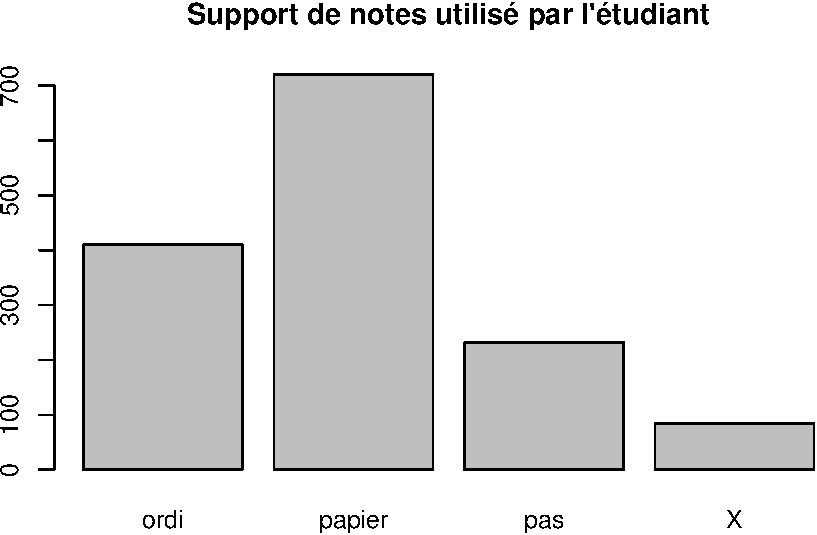
\includegraphics{qs_etudiants_files/figure-latex/Q1-1.pdf}
\end{figure}

\subsection{Q2- Pendant ce cours, vous avez complété la prise de notes
par (plusieurs réponses
possibles)}\label{q2--pendant-ce-cours-vous-avez-complete-la-prise-de-notes-par-plusieurs-reponses-possibles}

La variable Q2.5 est anormale. Il ne peut y avoir dans la même colonne
du texte et des nombres. La colonne ne peut contenir que 1 ou NA. Créer
une colnne supplémentaire pour le texte. Par ex. Q2-7.

\begin{figure}[htbp]
\centering
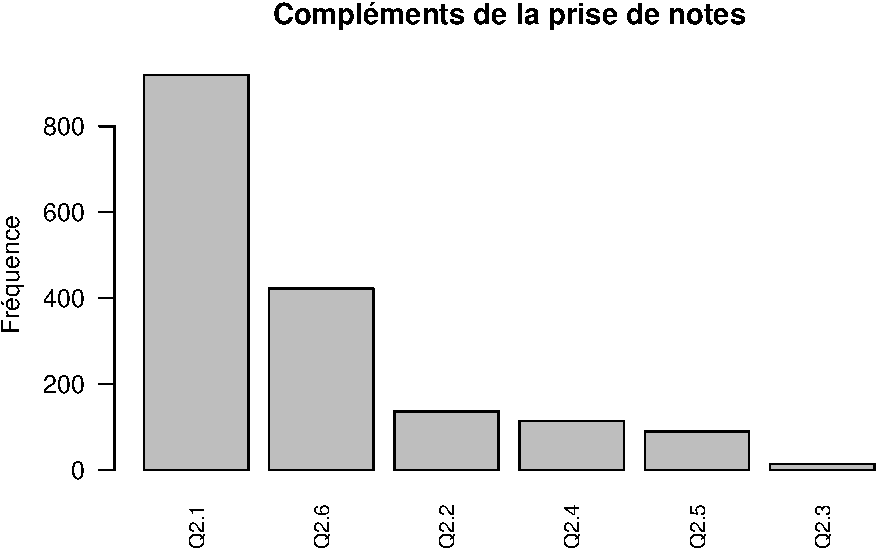
\includegraphics{qs_etudiants_files/figure-latex/unnamed-chunk-3-1.pdf}
\end{figure}

\begin{verbatim}
              0       1      2     3    4
nombre     8.00 1201.00 218.00 17.00 2.00
proportion 0.55   83.06  15.08  1.18 0.14
\end{verbatim}

\begin{figure}[htbp]
\centering
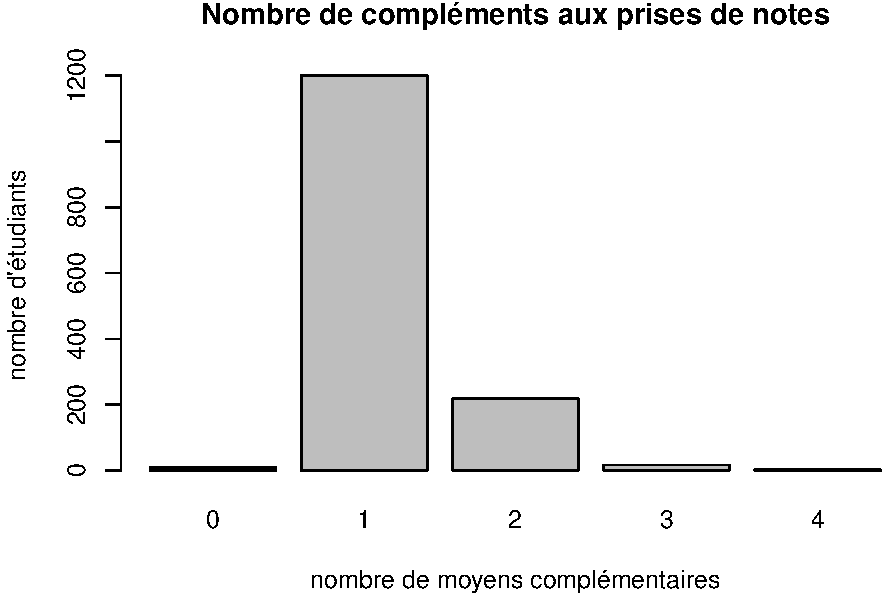
\includegraphics{qs_etudiants_files/figure-latex/unnamed-chunk-3-2.pdf}
\end{figure}

\subsection{Q3- Quels sont les outils numériques que vous aviez avec
vous pendant ce cours? (plusieurs réponses
possibles)}\label{q3--quels-sont-les-outils-numeriques-que-vous-aviez-avec-vous-pendant-ce-cours-plusieurs-reponses-possibles}

Colonnes 11 à 14

\paragraph{téléphone portable
classique}\label{telephone-portable-classique}

colonnes 10: ():non, oui sur la table= ot, oui dans mon sac ou ma poche=
osp

\begin{figure}[htbp]
\centering
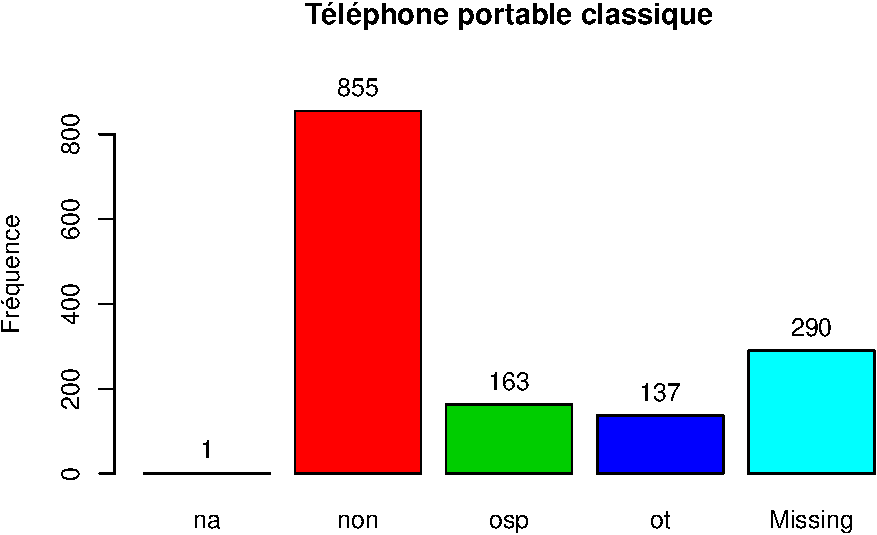
\includegraphics{qs_etudiants_files/figure-latex/outils-1.pdf}
\end{figure}

\begin{verbatim}
d1$Q3.1tpc : 
        Frequency   %(NA+)   %(NA-)
non           855     59.1     74.0
osp           163     11.3     14.1
ot            137      9.5     11.9
<NA>          291     20.1      0.0
  Total      1446    100.0    100.0
\end{verbatim}

\begin{figure}[htbp]
\centering
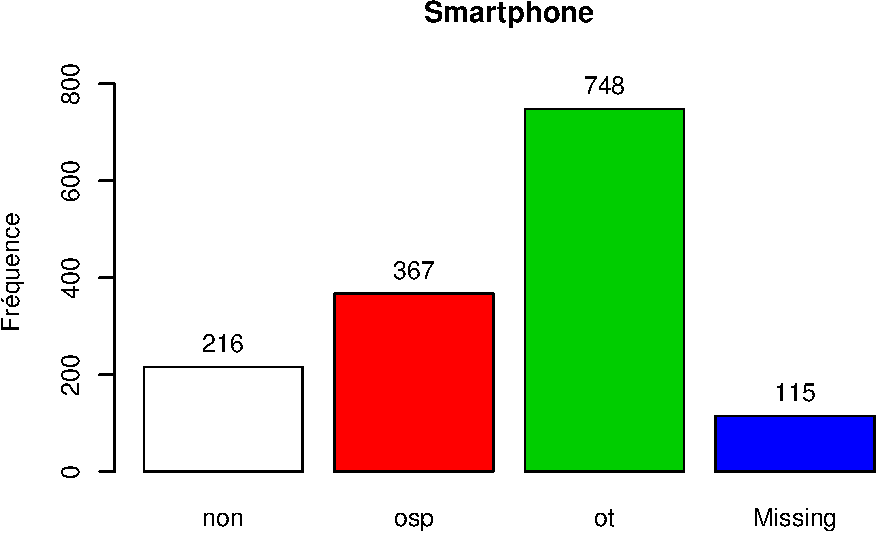
\includegraphics{qs_etudiants_files/figure-latex/outils-2.pdf}
\end{figure}

\begin{verbatim}
d1$Q3.2sp : 
        Frequency   %(NA+)   %(NA-)
non           216     14.9     16.2
osp           367     25.4     27.6
ot            748     51.7     56.2
<NA>          115      8.0      0.0
  Total      1446    100.0    100.0
\end{verbatim}

\begin{figure}[htbp]
\centering
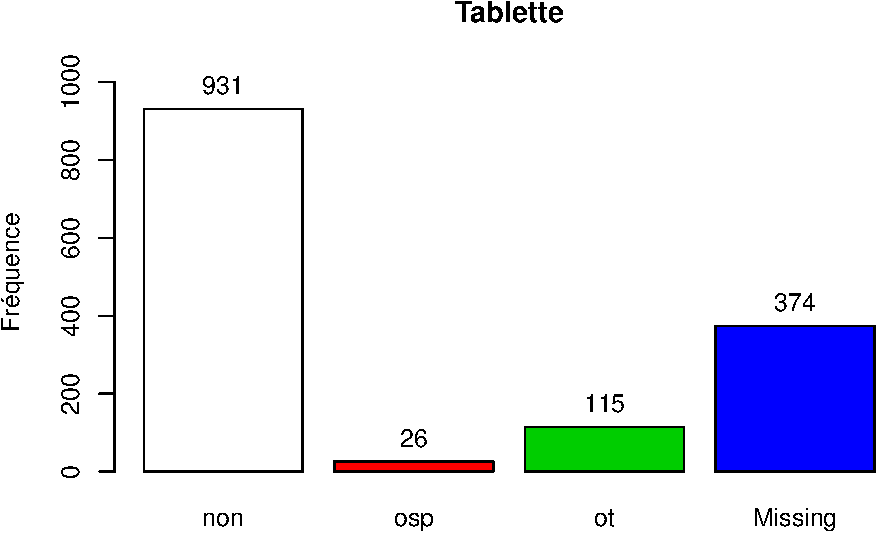
\includegraphics{qs_etudiants_files/figure-latex/outils-3.pdf}
\end{figure}

\begin{verbatim}
d1$Q3.3tab : 
        Frequency   %(NA+)   %(NA-)
non           931     64.4     86.8
osp            26      1.8      2.4
ot            115      8.0     10.7
<NA>          374     25.9      0.0
  Total      1446    100.0    100.0
\end{verbatim}

\begin{figure}[htbp]
\centering
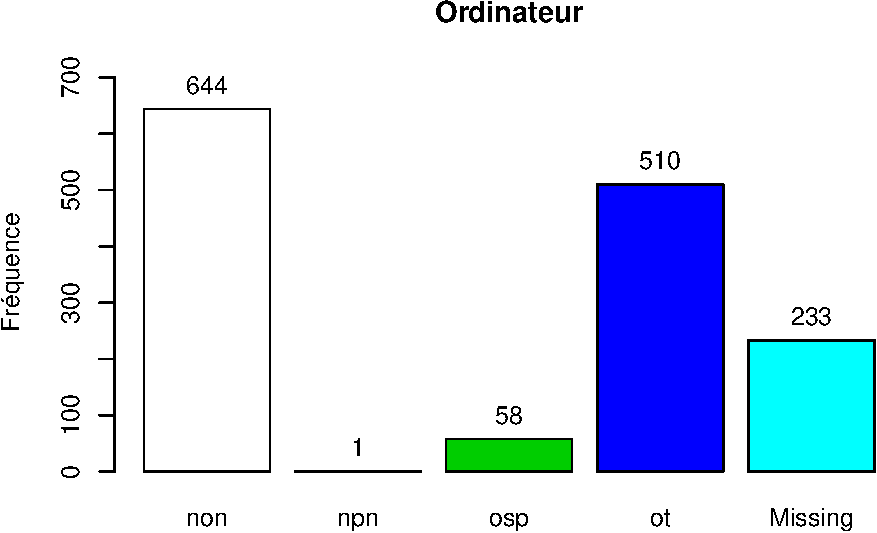
\includegraphics{qs_etudiants_files/figure-latex/outils-4.pdf}
\end{figure}

\begin{verbatim}
d1$Q3.4ord : 
        Frequency   %(NA+)   %(NA-)
non           644     44.5     53.1
npn             1      0.1      0.1
osp            58      4.0      4.8
ot            510     35.3     42.0
<NA>          233     16.1      0.0
  Total      1446    100.0    100.0
\end{verbatim}

\subsection{Q4- Pendant ce cours (en dehors des temps de pause
éventuels), vous avez utilisé votre téléphone pour (plusieurs réponses
possibles):}\label{q4--pendant-ce-cours-en-dehors-des-temps-de-pause-eventuels-vous-avez-utilise-votre-telephone-pour-plusieurs-reponses-possibles}

question 15 à 30

\begin{Shaded}
\begin{Highlighting}[]
\NormalTok{d1 <-}\StringTok{ }\KeywordTok{read.csv}\NormalTok{(}\KeywordTok{paste0}\NormalTok{(path, file1), }\DataTypeTok{skip =} \DecValTok{1}\NormalTok{, }\DataTypeTok{stringsAsFactors =} \OtherTok{FALSE}\NormalTok{)}

\NormalTok{q4 <-}\StringTok{ }\NormalTok{d1[, }\KeywordTok{c}\NormalTok{(}\DecValTok{15}\NormalTok{:}\DecValTok{26}\NormalTok{, }\DecValTok{28}\NormalTok{:}\DecValTok{30}\NormalTok{)]}
\NormalTok{q4 <-}\StringTok{ }\KeywordTok{as.data.frame}\NormalTok{(}\KeywordTok{sapply}\NormalTok{(q4,gsub,}\DataTypeTok{pattern=}\StringTok{"NR"}\NormalTok{,}\DataTypeTok{replacement=}\StringTok{"NA"}\NormalTok{), , }\DataTypeTok{stringsAsFactors =} \OtherTok{FALSE}\NormalTok{)}
\NormalTok{q4 <-}\StringTok{ }\KeywordTok{as.data.frame}\NormalTok{(}\KeywordTok{sapply}\NormalTok{(q4, as.integer))}
\NormalTok{a <-}\StringTok{ }\KeywordTok{apply}\NormalTok{(q4,}\DecValTok{2}\NormalTok{,sum, }\DataTypeTok{na.rm =} \OtherTok{TRUE}\NormalTok{)}
\NormalTok{x <-}\StringTok{ }\KeywordTok{barplot}\NormalTok{(}\KeywordTok{sort}\NormalTok{(a, }\DataTypeTok{decreasing =} \OtherTok{TRUE}\NormalTok{), }\DataTypeTok{las =} \DecValTok{2}\NormalTok{, }\DataTypeTok{main =} \StringTok{"Utilisation du téléphone pendant le cours"}\NormalTok{)}
\NormalTok{v <-}\StringTok{ }\KeywordTok{paste0}\NormalTok{(}\KeywordTok{sort}\NormalTok{(}\KeywordTok{round}\NormalTok{(a*}\DecValTok{100}\NormalTok{/}\KeywordTok{sum}\NormalTok{(a), }\DecValTok{2}\NormalTok{), }\DataTypeTok{decreasing =} \OtherTok{TRUE}\NormalTok{), }\StringTok{"%"}\NormalTok{)}
\KeywordTok{text}\NormalTok{(x, }\DecValTok{100}\NormalTok{, v, }\DataTypeTok{srt=}\DecValTok{90}\NormalTok{, }\DataTypeTok{cex =} \FloatTok{0.8}\NormalTok{)}
\end{Highlighting}
\end{Shaded}

\begin{figure}[htbp]
\centering
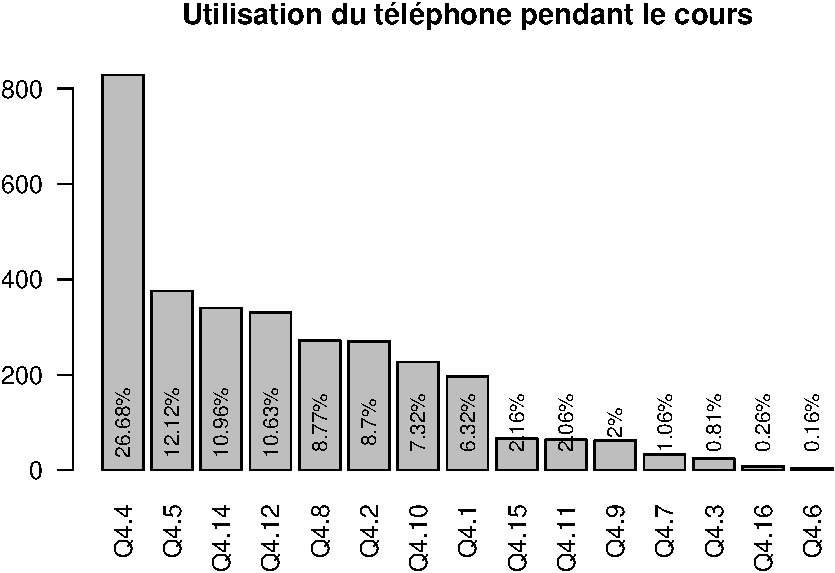
\includegraphics{qs_etudiants_files/figure-latex/Q4-1.pdf}
\end{figure}

Combien d'actions simultannément:

\begin{verbatim}
   Min. 1st Qu.  Median    Mean 3rd Qu.    Max. 
  0.000   1.000   2.000   2.146   3.000  12.000 
\end{verbatim}

\begin{verbatim}
  0   1   2   3   4   5   6   7   8  11  12 
 42 635 311 207 122  74  31  18   4   1   1 
\end{verbatim}

\begin{figure}[htbp]
\centering
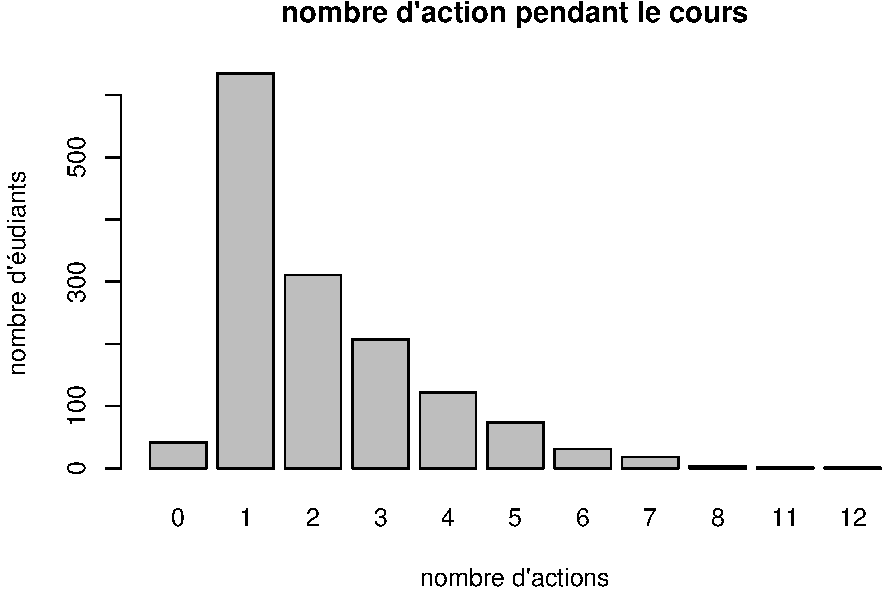
\includegraphics{qs_etudiants_files/figure-latex/actions_sim-1.pdf}
\end{figure}

\subsection{Q5- A quelle fréquence, avez-vous utilisé votre téléphone
PENDANT ce cours (en dehors des temps de pause éventuels) pour prendre
des notes ou chercher sur internet des informations au sujet du cours
?}\label{q5--a-quelle-frequence-avez-vous-utilise-votre-telephone-pendant-ce-cours-en-dehors-des-temps-de-pause-eventuels-pour-prendre-des-notes-ou-chercher-sur-internet-des-informations-au-sujet-du-cours}

question 31

\begin{verbatim}
  1X  jjs jnsp   js   na   NR  nvp  qqf   sv   tt NA's 
 136    1    9  835    6   66   11  251   64    9   58 
\end{verbatim}

\begin{figure}[htbp]
\centering
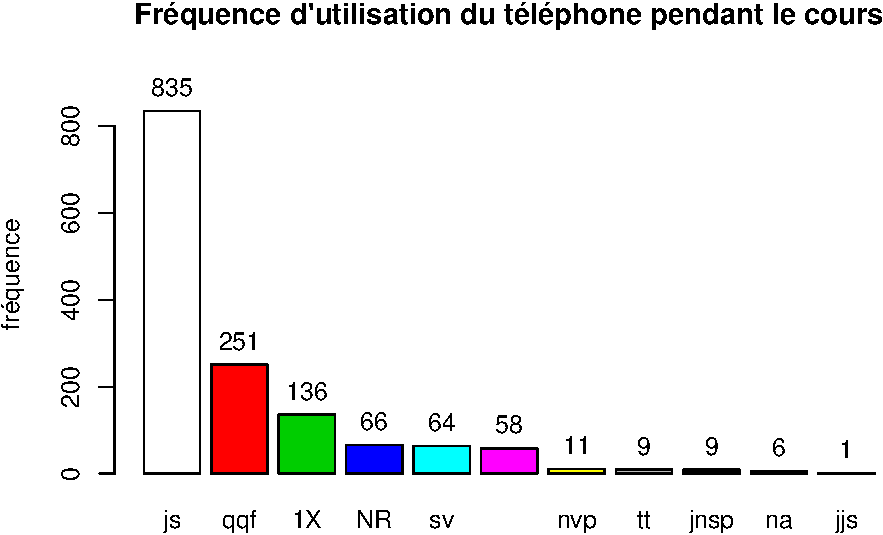
\includegraphics{qs_etudiants_files/figure-latex/utilisation-1.pdf}
\end{figure}

\begin{verbatim}
as.factor(d1$Q5) : 
        Frequency   %(NA+)   %(NA-)
js            835     57.7     60.2
qqf           251     17.4     18.1
1X            136      9.4      9.8
NR             66      4.6      4.8
sv             64      4.4      4.6
NA's           58      4.0      0.0
nvp            11      0.8      0.8
jnsp            9      0.6      0.6
tt              9      0.6      0.6
na              6      0.4      0.4
jjs             1      0.1      0.1
  Total      1446    100.0    100.0
\end{verbatim}

\subsection{Q6- A quelle fréquence, avez-vous utilisé votre téléphone
PENDANT ce cours (en dehors des temps de pause éventuels) pour faire
autre chose que prendre des notes ou chercher sur internet des
informations au sujet du
cours?}\label{q6--a-quelle-frequence-avez-vous-utilise-votre-telephone-pendant-ce-cours-en-dehors-des-temps-de-pause-eventuels-pour-faire-autre-chose-que-prendre-des-notes-ou-chercher-sur-internet-des-informations-au-sujet-du-cours}

question 32

\begin{verbatim}
  1X jnsp   js   na   NR  nvp  qqf   sv   tt NA's 
 183    5  303    3   67   16  524  242   45   58 
\end{verbatim}

\begin{figure}[htbp]
\centering
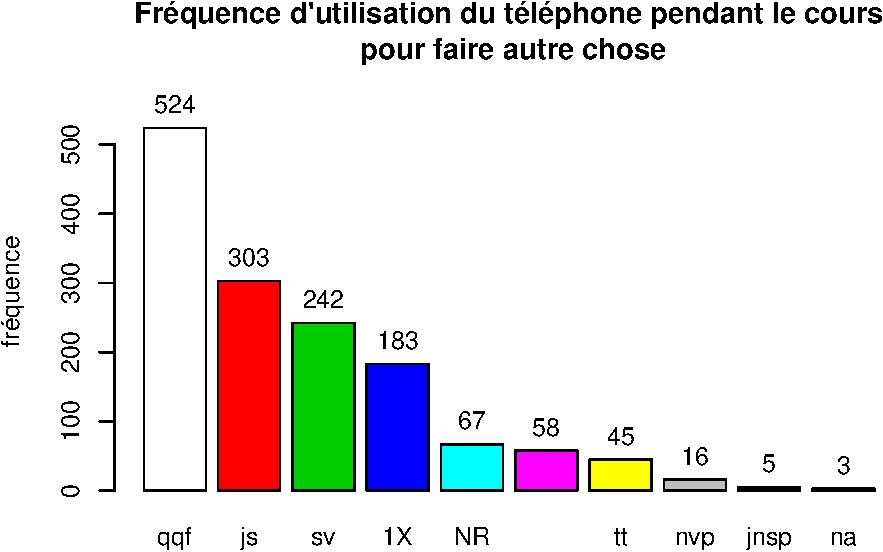
\includegraphics{qs_etudiants_files/figure-latex/utilisation2-1.pdf}
\end{figure}

\begin{verbatim}
as.factor(d1$Q6) : 
        Frequency   %(NA+)   %(NA-)
qqf           524     36.2     37.8
js            303     21.0     21.8
sv            242     16.7     17.4
1X            183     12.7     13.2
NR             67      4.6      4.8
NA's           58      4.0      0.0
tt             45      3.1      3.2
nvp            16      1.1      1.2
jnsp            5      0.3      0.4
na              3      0.2      0.2
  Total      1446    100.0    100.0
\end{verbatim}

\subsection{Q7- Pendant ce cours (en dehors des temps de pause
éventuels), vous avez utilisé votre tablette et/ ou votre ordinateur
pour (plusieurs réponses
possibles):}\label{q7--pendant-ce-cours-en-dehors-des-temps-de-pause-eventuels-vous-avez-utilise-votre-tablette-et-ou-votre-ordinateur-pour-plusieurs-reponses-possibles}

Questions 33 à 48

\begin{verbatim}
[1] "Analyse de la colonne Q7.13 (réponse libre)"
\end{verbatim}

\begin{verbatim}
                            1          cours  dessinerpaint        docmail 
          1335              1              1              1              1 
      frfiches    inscrcourse        Lemotiv           lire     notercours 
             1              1              1              3             39 
   orgdossinfo            ppt       pptcours         prepCV  reg_autr_cour 
             1              1              3              2              1 
  reg_pptander      reg-heure     reg-photos        reg-ppt regautre cours 
             1              1              1              1              1 
      regcours         regppt           shop    suivrecours        support 
             1              1              3              1              1 
 telecharcours            TFE           word           WTFE           NA's 
             1              3              1              1             36 
\end{verbatim}

\begin{figure}[htbp]
\centering
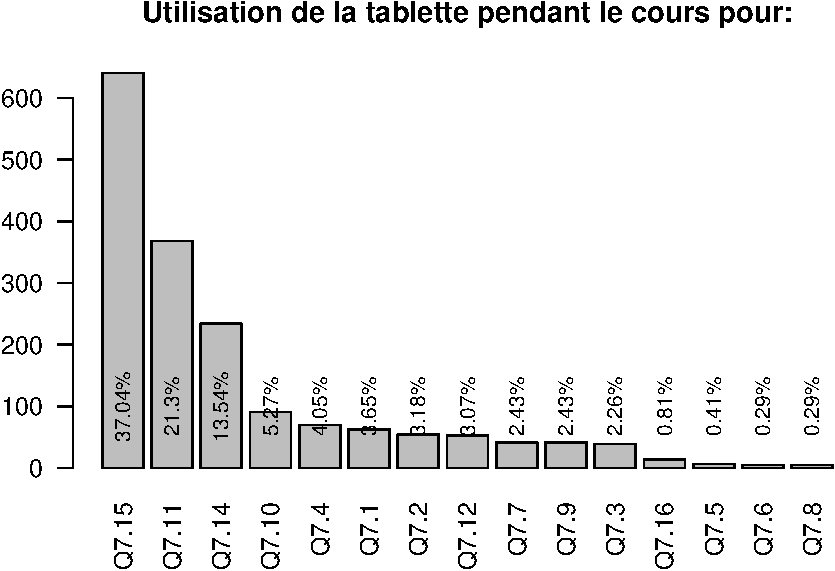
\includegraphics{qs_etudiants_files/figure-latex/q7-1.pdf}
\end{figure}

\subsection{Q8- A quelle fréquence, avez-vous utilisé votre tablette,
et/ ou votre ordinateur PENDANT ce cours (en dehors des temps de pause
éventuels) pour prendre des notes ou chercher sur internet des
informations au sujet du cours
?}\label{q8--a-quelle-frequence-avez-vous-utilise-votre-tablette-et-ou-votre-ordinateur-pendant-ce-cours-en-dehors-des-temps-de-pause-eventuels-pour-prendre-des-notes-ou-chercher-sur-internet-des-informations-au-sujet-du-cours}

question 49
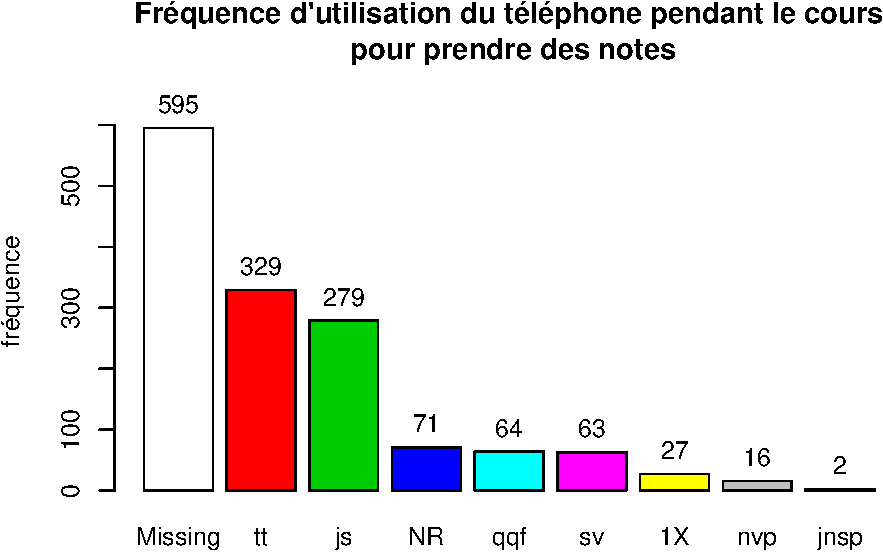
\includegraphics{qs_etudiants_files/figure-latex/utilisatin3-1.pdf}

\begin{verbatim}
as.factor(d1$Q8) : 
        Frequency   %(NA+)   %(NA-)
NA's          595     41.1      0.0
tt            329     22.8     38.7
js            279     19.3     32.8
NR             71      4.9      8.3
qqf            64      4.4      7.5
sv             63      4.4      7.4
1X             27      1.9      3.2
nvp            16      1.1      1.9
jnsp            2      0.1      0.2
  Total      1446    100.0    100.0
\end{verbatim}

\subsection{Q9- A quelle fréquence, avez-vous utilisé votre tablette,
et/ ou votre ordinateur PENDANT ce cours (en dehors des temps de pause
éventuels) pour faire autre chose que prendre des notes ou chercher sur
internet des informations au sujet du cours
?}\label{q9--a-quelle-frequence-avez-vous-utilise-votre-tablette-et-ou-votre-ordinateur-pendant-ce-cours-en-dehors-des-temps-de-pause-eventuels-pour-faire-autre-chose-que-prendre-des-notes-ou-chercher-sur-internet-des-informations-au-sujet-du-cours}

question 50

\begin{figure}[htbp]
\centering
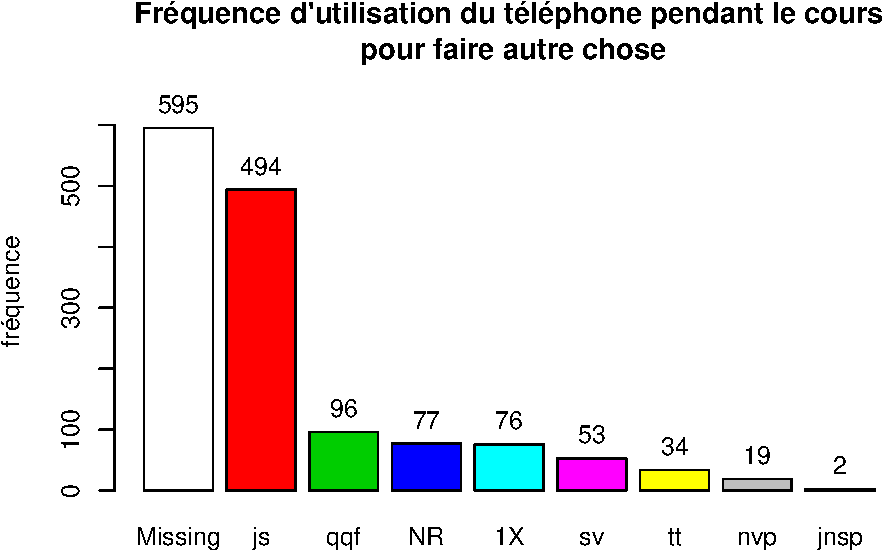
\includegraphics{qs_etudiants_files/figure-latex/utilisation4-1.pdf}
\end{figure}

\begin{verbatim}
as.factor(d1$Q9) : 
        Frequency   %(NA+)   %(NA-)
NA's          595     41.1      0.0
js            494     34.2     58.0
qqf            96      6.6     11.3
NR             77      5.3      9.0
1X             76      5.3      8.9
sv             53      3.7      6.2
tt             34      2.4      4.0
nvp            19      1.3      2.2
jnsp            2      0.1      0.2
  Total      1446    100.0    100.0
\end{verbatim}

\section{Information de session}\label{information-de-session}

Informations pour le chapitre matériel et méthode.

\begin{verbatim}
R version 3.1.3 (2015-03-09)
Platform: x86_64-apple-darwin13.4.0 (64-bit)
Running under: OS X 10.10.3 (Yosemite)

locale:
[1] fr_FR.UTF-8/fr_FR.UTF-8/fr_FR.UTF-8/C/fr_FR.UTF-8/fr_FR.UTF-8

attached base packages:
[1] stats     graphics  grDevices utils     datasets  methods   base     

other attached packages:
[1] knitr_1.10       xtable_1.7-4     stringr_1.0.0    epicalc_2.15.1.0
[5] nnet_7.3-9       MASS_7.3-40      survival_2.38-1  foreign_0.8-63  

loaded via a namespace (and not attached):
 [1] digest_0.6.8      evaluate_0.7      formatR_1.2      
 [4] htmltools_0.2.6   magrittr_1.5      rmarkdown_0.5.3.2
 [7] splines_3.1.3     stringi_0.4-1     tools_3.1.3      
[10] yaml_2.1.13      
\end{verbatim}

\begin{verbatim}

To cite R in publications use:

  R Core Team (2015). R: A language and environment for
  statistical computing. R Foundation for Statistical Computing,
  Vienna, Austria. URL http://www.R-project.org/.

A BibTeX entry for LaTeX users is

  @Manual{,
    title = {R: A Language and Environment for Statistical Computing},
    author = {{R Core Team}},
    organization = {R Foundation for Statistical Computing},
    address = {Vienna, Austria},
    year = {2015},
    url = {http://www.R-project.org/},
  }

We have invested a lot of time and effort in creating R, please
cite it when using it for data analysis. See also
'citation("pkgname")' for citing R packages.
\end{verbatim}

\end{document}
